\documentclass{article}
\usepackage{graphicx}
\usepackage{caption}
\usepackage{subcaption}
\usepackage{amsmath}
\usepackage{amssymb}
\usepackage{anysize}
\marginsize{2,7cm}{2,7cm}{2cm}{3cm}
\usepackage[french]{babel}
\usepackage[utf8]{inputenc}
\graphicspath{{image/}}
%%%%%%%%%%%%%%%% Lengths %%%%%%%%%%%%%%%%
\setlength{\textwidth}{15.5cm}
\setlength{\evensidemargin}{0.5cm}
\setlength{\oddsidemargin}{0.5cm}

%%%%%%%%%%%%%%%% Variables %%%%%%%%%%%%%%%%
\def\projet{2}
\def\titre{Résolution de systèmes linéaires et application à l'équation de la chaleur}
\def\groupe{2}
\def\equipe{12417}
\def\responsible{jmeurgues}
\def\secretary{mbelamrabet}
\def\others{lguerin005, alamhamdi001, tpitault}

\begin{document}

%%%%%%%%%%%%%%%% Header %%%%%%%%%%%%%%%%
\noindent\begin{minipage}{0.98\textwidth}
  \vskip 0mm
  \noindent
  { \begin{tabular}{p{7.5cm}}
      {\bfseries \sffamily
        Projet \projet} \\ 
      {\itshape \titre}
    \end{tabular}}
  \hfill 
  \fbox{\begin{tabular}{l}
      {~\hfill \bfseries \sffamily Groupe \groupe\ - Equipe \equipe
        \hfill~} \\[2mm] 
      Responsable : \responsible \\
      Secrétaire : \secretary \\
      Codeurs : \others
    \end{tabular}}
  \vskip 4mm ~

  ~~~\parbox{0.95\textwidth}{\small \textit{Résumé~:} La résolution de systèmes linéaires est un problème courant et présent dans de nombreux domaines de recherche comme la diffusion de chaleur. Cette résolution se fait sur des systèmes de taille conséquente pouvant contenir des milliers d'équations. Plusieurs méthodes de résolution existent telle que la méthode du pivot de Gauss. Bien que nous sachions résoudre beaucoup de ces systèmes d'équations, deux autres problèmes se posent, celui de la résolution en un temps raisonnable et celui de la place mémoire occupée par le problème. Nous allons nous consacrer dans une première partie à la méthode de la factorisation de Cholesky adaptée à certains systèmes linaires. Puis nous étudierons une seconde méthode appelée méthode du gradient conjugué. Pour finir nous appliquerons une partie de nos méthodes de résolution de systèmes pour résoudre des cas particuliers du problème de diffusion de la chaleur en deux dimensions \sffamily  }
  \vskip 1mm ~
\end{minipage}

%%%%%%%%%%%%%%%% Main part %%%%%%%%%%%%%%%%

\section{Décomposition de Cholesky}

\textit{La documentation complète du projet est décrite dans le fichier \texttt{refman.pdf} ou accessible via \texttt{index.html}. Toutes les fonctions présentées dans cette partie ainsi que leurs tests structurels sont implémentés dans les fichiers contenus dans le dossier \texttt{partie\_1}. S'y trouvent également leur documentation et leur complexité, accessibles avec la commande \texttt{help(fonction)} de la console python.}
\vspace{10pt}

La décomposition de Cholesky est une décomposition privilégiée pour diminuer le temps de résolution d'un système linéaire qui peut se mettre sous la forme $Ax=b$ avec $A$ une matrice symétrique définie positive. Une matrice symétrique définie positive est une matrice symétrique dont les valeurs propres sont strictement positives. Pour simplifier la résolution d'un système linéaire $Ax=b$, la décomposition de Cholesky transforme la matrice $A$ en un produit $T\cdot~^tT$. La matrice $T$ est alors une matrice triangulaire inférieure. Ses coefficients se calculent selon les formules suivantes :\\
\[ \left\{
\begin{array}{rcr}
  t_{i,i}^{2} & = & a_{i,i} - \sum\limits^{i-1}_{k=1}t_{i,k}^{2} \mbox{ } \mbox{ } \mbox{ } \mbox{ }\mbox{ } \mbox{ } \mbox{ } \mbox{ } \mbox{ } \mbox{ } \mbox{ } \mbox{ } \\
  t_{j,i} & = & \dfrac{a_{i,j} - \sum\limits^{i-1}_{k=1}t_{i,k}t_{j,k}}{t_{i,i}} \mbox{ } j > i \\
\end{array}
\right.\]

Pour commencer nous avons implémenté les fonctions \texttt{calc\_ti} et \texttt{calc\_tji} contenues dans le fichier \texttt{partie1\_q1.py} qui vont respectivement calculer les termes \texttt{$t_{i,i}$} et \texttt{$t_{j,i}$} et retourner leur valeur. Pour cela, la fonction \texttt{calc\_ti} prend en argument la matrice $A$ de taille $n \times n$ à factoriser, la matrice $T$ supposée complétée pour les termes nécessaires au calcul de $t_{i,i}$ ainsi que le paramètre \texttt{i}. L'exécution de la fonction comprend \texttt{i-1} additions, \texttt{i-1} multiplications et un calcul de racine carrée supposé constant, donc cette exécution se fait en \texttt{(2i-1)} opérations élémentaires. Pour la fonction \texttt{calc\_tji} nous prenons un paramètre supplémentaire qui est \texttt{j}. Le calcul s'effectue lui aussi en \texttt{(2i-1)} opérations élémentaires. Nous avons testé ces deux fonctions sur différentes matrices $A$ symétriques définies positives et avec des matrices $T$ partiellement complétées avec les valeurs théoriques.

Ensuite nous avons codé une fonction \texttt{facto\_cholesky\_dense} qui prend une matrice $A$ symétrique définie positive de taille $n\times n$, et qui retourne sa décomposition de Cholesky. Pour cela la fonction fait appel à une fonction auxiliaire \texttt{facto\_cholesky\_dense\_REC} qui fait \texttt{n} appels récursifs sur les différents termes à calculer de la matrice $T$, initialisée à la matrice nulle. Au total la fonction effectue \texttt{1} appel sur la fonction \texttt{calc\_ti} et \texttt{(n-i-1)} appels sur la fonction \texttt{calc\_tji} soit \texttt{(n-i)(2i-1)} opérations élémentaires par appel à la fonction \texttt{facto\_cholesky\_dense\_REC}. Le nombre d'opérations élémentaires de notre fonction principale \texttt{facto\_cholesky\_dense} effectuant \texttt{n} appels sur notre fonction récursive est alors :
\begin{center}
  $\displaystyle{\sum\limits^{n}_{i=1}(n-i)(2i-1) = \dfrac{1}{6}\begin{pmatrix}n(n+1)(2n+1)-6n^{2}\end{pmatrix} \underset{+\infty}{\approx} \dfrac{1}{3}n^{3}}$
\end{center}
La compléxité totale de notre algorithme de factorisation de Cholesky est de l'ordre de $\dfrac{1}{3}n^{3}$. En factorisant $A$ le système $Ax=b$ devient $T~^tTx=b$ avec $T$ une matrice triangulaire inférieure de taille $n \times n$. Pour résoudre ce système, il suffit de trouver d'abord le vecteur \texttt{y} tel que $Ty=b$ qui se fait en un temps de l'ordre de \texttt{$n^{2}$}. Puis de trouver à partir de ce vecteur calculé le vecteur \texttt{x} tel que $~^{t}Tx=y$ qui se résout aussi en un temps de l'ordre de \texttt{$n^{2}$}. Au final la résolution du système linéaire $Ax=b$ avec $A$ symétrique définie positive se fait en un temps de l'ordre de $\dfrac{1}{3}n^{3}+O(n^{2})$ contre $0(n!)$ avec une méthode classique ce qui est non négligeable.\\

En revanche, la méthode de factorisation de Cholesky est coûteuse en temps quand la matrice $A$ est creuse, c'est-à-dire quand le nombre de coefficients extra-diagonnaux non nul de $A$. Dans cette situation le calcul de certains coefficients de la matrice résultante de la décomposition est inutile. Il existe une factorisation dite incomplète qui calcule uniquement $t_{j,i}$ si $a_{i,j}$ est non nul. Pour vérifier l'efficacité de cette méthode dans le cas où $A$ est creuse, nous souhaitons confronter le temps d'exécution des deux méthodes de factorisaton. Pour commencer, nous avons implémenté une fonction \texttt{generate\_SPDSM} qui prend en entrée un entier \texttt{n} et un entier pair positif ou nul \texttt{i} et qui retourne une matrice symétrique définie positive creuse de taille $n^{2}$ avec $i$ coefficients extra-diagonnaux non nuls. Ensuite, nous avons codé l'algorithme de factorisation de Cholesky incomplète en reprenant notre premier algorithme et en y ajoutant la condition de calcul de $t_{j,i}$ si $a_{j,i}$ est non nul.

Les premiers tests que nous avons réalisé ont été de vérifier si le résultat obtenu par les deux méthodes était identique à un certain de seuil de précision pour une même matrice $A$ creuse. Puis nous avons testé la différence de temps d'exécution entre les deux méthodes sur des matrices générées aléatoirement, à l'aide de la fonction \texttt{generate\_SPDSM}. La figure ~\ref{fig:comparaison_facto} illustre la différence de temps d'éxécution pour des matrices de tailles variables et dont le nombre de coefficients extra-diagonaux non nuls est égal à la taille de la matrice. De plus nous pouvons constater un gain de temps pour la factorisation incomplète.

\begin{figure}[htbp]
  \centering
  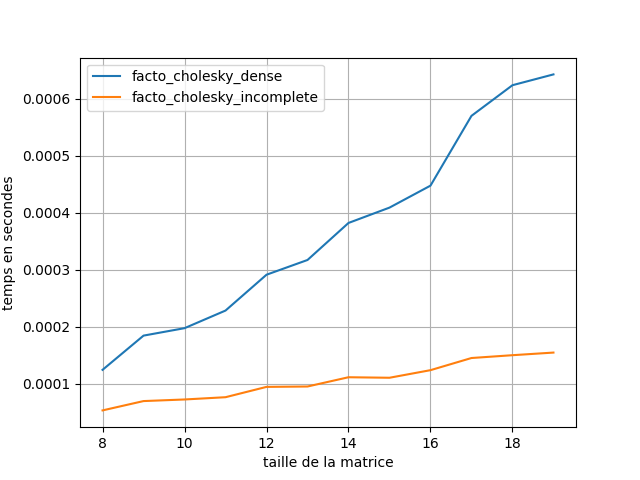
\includegraphics[width=0.5\textwidth]{images/Graphe.png}
  \caption{Comparaison du temps d'exécution des deux méthodes de factorisation de Cholesky (dense et incomplète).}
  \label{fig:comparaison_facto}
\end{figure}% 

En effet, pour la factorisation de Cholesky incomplète, si l'on prend en paramètre \texttt{n} la taille de la matrice donnée en entrée et \texttt{c} le nombre de coefficients extra-diagonaux non nuls, nous avons un total de \texttt{(2i-1)} opérations pour les \texttt{n} coefficients diagonaux, $\dfrac{c}{2}$ calculs de coefficients extra-diagonnaux coûtant chacun \texttt{(2i-1)} opérations. En moyenne nous avons donc $(\dfrac{c}{2n}+1)(2i-1)$ opérations par appel. Le calcul de complexité devient :
\begin{center}
  $\displaystyle{\sum\limits^{n}_{i=1}(1+\dfrac{c}{2n})(2i-1)\underset{+\infty}{\approx}(1+\dfrac{c}{2n})n^{2}}$
\end{center}

La complexité de la factorisation imcomplète de Cholesky est meilleure dans le cas creux que celle de la factorisation dense car le paramètre \texttt{c} est supposé très petit devant le nombre total de termes extra-diagonnaux. On peut gagner jusqu'à un facteur $\dfrac{1}{3}n$ ce qui est non négligeable pour des matrices de tailles importantes. De plus pour la résolution des équations $Ty=b$ et $~^{t}Tx=y$ cela se fait en un temps linéaire en le nombre de coefficients extra-diagonaux non nuls. La résolution d'un système linéaire avec la factorisation incomplète aura donc une complexité de l'ordre de $O((1+\dfrac{c}{2n})n^{2})$. La décomposition incomplète peut aussi permettre un gain de stockage de données en implémentant une structure spécifique aux matrices creuses en ne gardant en mémoire que les coefficients non nuls et leurs indices.\\

Enfin, nous avons créé une fonction \texttt{est\_bon\_preconditionneur} qui prend en argument deux  matrices $T$ et $A$ et qui vérifie si $T.^tT$ est un bon préconditionneur de $A$; c'est à dire qu'il vérifie :
\begin{center}
  $\displaystyle{cond(^tT^{-1}.T^{-1}.A) < cond(A)}$
\end{center}
Nous avons testé cette fonction avec une matrice $A$ symétrique définie positive générée à l'aide de la fonction \texttt{generate\_SPDSM} et de la matrice triangulaire inférieure $T$ obtenue grâce aux deux méthodes de décomposition de Cholesky : $A = T.^tT$.

\section{Méthode du gradient conjugué}

\textit{Toutes les fonctions présentées dans cette partie ainsi que leurs tests structurels sont implémentés dans les fichiers contenus dans le dossier \texttt{partie\_2}. S'y trouvent également leur documentation et leur complexité, accessibles avec la commande \texttt{help(fonction)} de la console python.}
\vspace{10pt}

Dans cette partie, on s'interesse à la méthode du gradient conjugué. C'est une autre méthode destinée à des systèmes linéaires $Ax=b$ où  $A$ est une matrice symétrique définie positive. Contrairement à la première méthode qui est directe, la méthode du gradient conjugué est une approximation du résultat souhaité, obtenue en un nombre fini d'itérations, et paramétrée par une initialisation possiblement astucieuse. En effet, dans certains problèmes, notamment physiques, une initialisation ressemblant à la solution peut-être intuitée. Malheureusement, dans le cas général, les méthodes pour trouver cette initialisation sont trop coûteuses, c'est pourquoi le vecteur nul est généralement utilisé.

Le principe de la méthode des gradients conjugués repose sur la décomposition en base orthogonale du minimiseur de la fonction f : 
\begin{center}
  $\displaystyle{f(x) = \dfrac{x^TAx}{2} - x^Tb}$
\end{center}
À chaque itération, l'algorithme détermine une nouvelle direction et un nouveau coefficient de la décomposition en base orthogonale de la solution et ajoute leur produit à la solution de l'itération précédente. Notre algorithme fait donc tendre une variable vers la solution recherchée. 

Dans un premier temps, nous avons mis en oeuvre la méthode des gradients conjugués dans la fonction \texttt{conjugate\_gradient}. Cette fonction, bien que fonctionnelle, possède plusieurs défauts. Tout d'abord, elle réalise une boucle $for$ qui utilise une valeur arbitrairement fixée à ${10^{6}}$, ce qui n'est pas idéal étant donée que l'on sait que l'algorithme à besoin de n itérations maximum. De plus, la précison souhaitée est elle aussi fixée dans le code et n'est pas paramétrable par l'utilisateur. Enfin la sortie de l'algorithme, lorqu'une précision suffisante est atteinte, se fait grâce à l'instruction $break$, ce qui n'est pas une pratique de codage saine. 

Dans un second temps, nous avons modifié la précédente implémentation de la méthode du gradient conjugué pour qu'elle utilise un préconditionneur obtenu à travers la décomposition incomplète de Cholesky. 

La figure ~\ref{fig:Nombre_iterations_Temps} montre une comparaison entre le nombre d'itérations et le temps pris par la méthode du gradient conjugué avec et sans préconditionnement, pour des matrices de dimensions différentes. Ces graphes ont été obtenus en générant des matrices symétriques définies positives creuses grâce à la fonction \texttt{generate\_SPDSM} écrite dans la partie 1.

Étant donné que la solution du problème est de dimension \texttt{n} et que l'on trouve une direction à chaque itération, l'algorithme termine en maximum \texttt{n} étapes. Il n'est donc pas surprenant que le nombre d'itérations pour chaque méthode présentée dans la figure ~\ref{fig:Nombre_iterations_Temps} soit dominé par la droite \texttt{y=N} avec \texttt{N} la dimension de la matrice en entrée. De plus, l'algorithme est prévu pour s'arrêter lorsque la précision souhaitée est atteinte. Le graphique représentant le nombre d'itérations figure ~\ref{fig:Nombre_iterations_Temps} permet de rendre compte du gain de temps occasioné par cet arrêt prématuré.

La figure ~\ref{fig:Nombre_iterations_Temps} montre aussi que le préconditionnement a un impact non négligeable sur le temps d'exécution de l'algorithme, temps grandement influencé par la double résolution de système réalisée à chaque itération. Pourtant, ce préconditionneur, bien que coûteux à obtenir, permet de faire converger l'algorithme en un nombre d'itérations bien moindre comparé à la première méthode, comme l'atteste la figure ~\ref{fig:Nombre_iterations_Temps}. Remarquons que la représentation des matrices sous forme de matrices creuses pourrait permettre un gain de temps considérable pour cet algorithme en supposant l'implémentation d'algorithmes de résolution de systèmes adaptés à cette représentation.

\begin{figure}[!htbp]
  \centering
  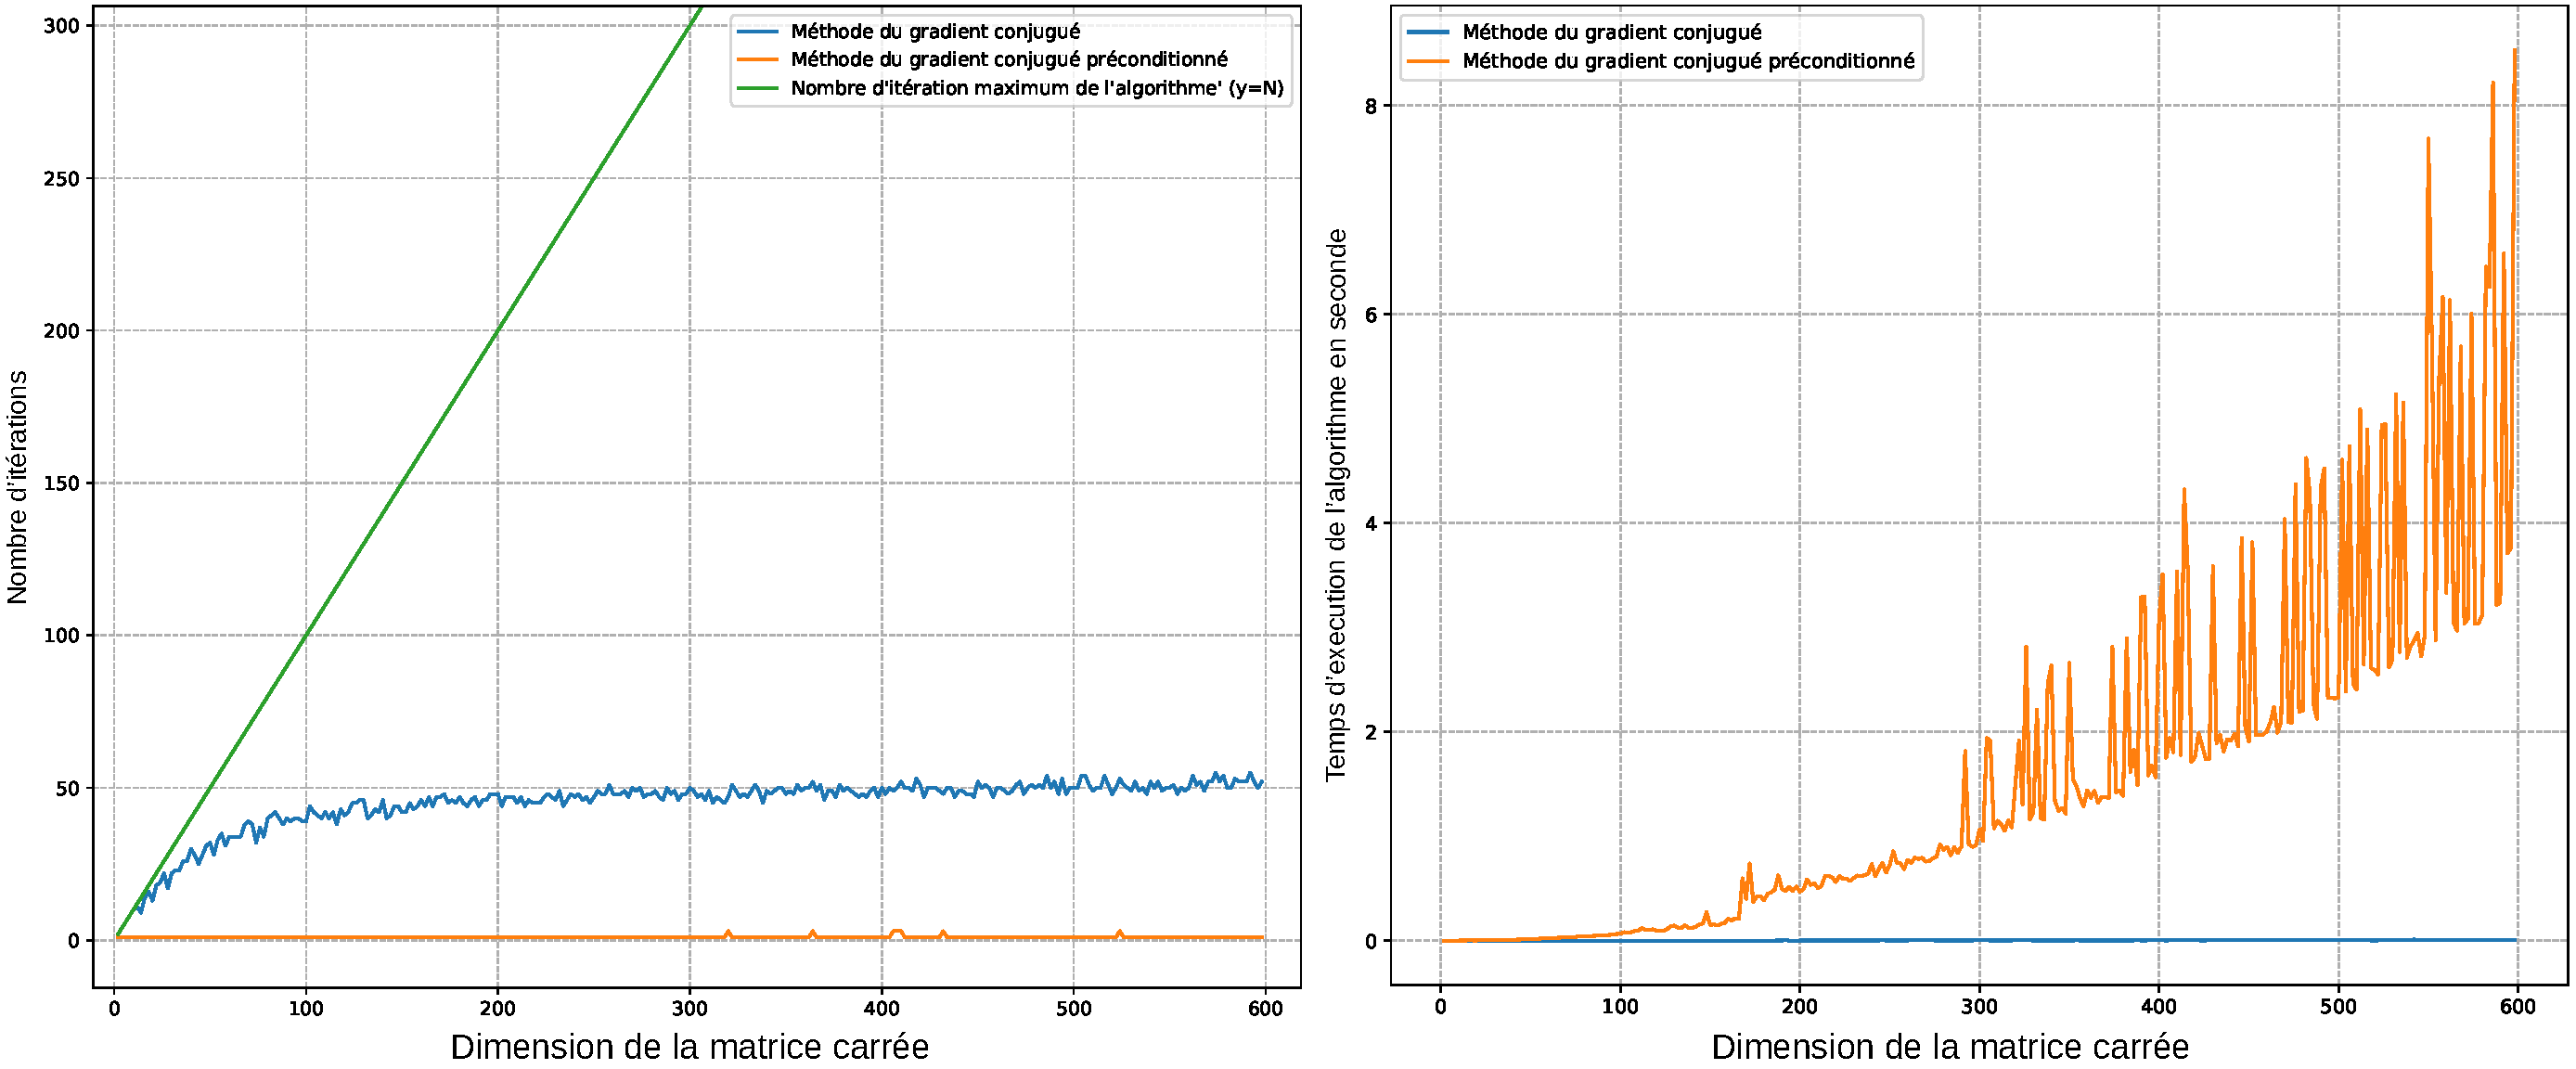
\includegraphics[width=0.90\textwidth]{images/Nombre_iterations_Temps.pdf}
  \caption{Comparaison du nombre d'itérations (à gauche) et du temps d'exécution (à droite) pour la méthode du gradient conjugué avec et sans préconditionnement} 
  \label{fig:Nombre_iterations_Temps}
\end{figure}

 

\section{Application à l'équation de la chaleur}

\textit{Toutes les fonctions présentées dans cette partie ainsi que leurs tests structurels sont implémentés dans les fichiers contenus dans le dossier \texttt{partie\_3}. S'y trouvent également leur documentation et leur complexité, accessibles avec la commande \texttt{help(fonction)} de la console python.}
\vspace{10pt}

Dans cette partie, on s'interesse à une application des deux méthodes traitées précédemment pour résoudre un système linéaire lié à l'équation de diffusion de la chaleur en mode stationnaire. Notre but est de calculer l'évolution de la température en chacun des points d'un plan représenté par un carré unitaire. Si on note $T(x,y)$ la température en un point du carré, et $f(x,y)$ l’apport de chaleur extérieur en ce même point, alors l’équation est la suivante :
$$\displaystyle{\frac{\partial^2 T}{\partial x^2} + \frac{\partial^2 T}{\partial y^2} + f(x,y)= \dfrac{\partial T}{\partial t} \quad \quad \forall(x,y) \in [0;1] \times [0;1]}$$

Pour les conditions aux limites sur les bords du domaine étudié nous prenons les conditions au bords de Dirichlet :

\[ \left\{
\begin{array}{rcr}
  T(0,y) =  T(1,y) =  0 & \forall y \in [0;1]\\
  T(x,0) = T(x,1)  =  0 & \forall x \in [0;1]\\
\end{array}
\right.\]

Comme nous considérons une évolution en mode stationnaire alors $\dfrac{\partial T}{\partial t} = 0$ et l'équation devient :

$$\displaystyle{\frac{\partial^2 T}{\partial x^2} + \frac{\partial^2 T}{\partial y^2} = -f(x,y) \quad \quad \forall(x,y) \in [0;1] \times [0;1]}$$


Étant donnée une fonction $f$, on cherche à trouver la fonction $T$ en appliquant la méthode des différences finies. C'est-à-dire en discrétisant notre plan en \texttt{$N\times N$} points répartis uniformément.

Dans notre cas $\Delta x$ et $\Delta y$ sont constants et seront égaux à $h=\dfrac{1}{N+1}$. La température discrète au point $(x_{i},y_{i})$  sera notée $T_{i,j}$. Une approximation des dérivés secondes de l'équation donne :
\[ \left\{
\begin{array}{rcr}
  
  \displaystyle{\begin{pmatrix} \dfrac{\partial^{2} T}{\partial x^{2}} \end{pmatrix}_{i,j}} & = &\displaystyle{\dfrac{T_{i+1,j} - 2T_{i,j} + T_{i-1,j}}{h^{2}}} \\
  \displaystyle{\begin{pmatrix} \dfrac{\partial^{2} T}{\partial y^{2}} \end{pmatrix}_{i,j}} & = & \displaystyle{\dfrac{T_{i,j+1} - 2T_{i,j} + T_{i,j-1}}{h^{2}}} \\
\end{array}
\right.\]

La formule discrétisée devient alors :

\begin{equation}
  \dfrac{1}{h^{2}}(-4T_{i,j} + T_{i+1,j} + T_{i-1,j} + T_{i,j+1} + T_{i,j-1} ) = -f(T_{i,j})
\end{equation}

On obtient alors l'équation matricielle :

\begin{equation}
  \Delta T = \dfrac{1}{h^{2}}A T = -f(T)
\end{equation}

Puis nous transformons cette équation en système linéaire :
\[ \left\{
\begin{array}{rcr}
  
  Ax & = & b \\
  b_{i*N+j} & = & -h^{2}\times f(T_{i,j}) \\
  x_{i*N+j} & = & T_{i,j} \\
\end{array}
\right.\]
En prenant $I_{N}$ la matrice identité de taille $N$ et en définissant $D$ de taille $N\times N$ par $\begin{pmatrix} -4 & 1 & 0 & 0 \\ 1 & \ddots & \ddots & 0 \\ 0 & \ddots & \ddots & 1  \\ 0  & 0 & 1 & -4 \end{pmatrix} $, on aura $A = \begin{pmatrix}  D & I_{N} & 0 & 0 \\ I_{N} & \ddots & \ddots & 0 \\ 0 & \ddots & \ddots & I_{N}  \\ 0  & 0 & I_{N} & D \end{pmatrix} $ une matrice tridiagonale de taille $N^{2}\times N^{2}$.




\subsection{Résolution du système dans le cas d'un mur chaud placé au nord}


Une fois notre système linéaire mis en place, nous avons souhaité le résoudre pour le cas d'un mur chaud placé au nord d'un espace non chauffé. Ainsi notre vecteur de conditions initiales \texttt{b}  devient :
\begin{equation}\displaystyle{
  b=\begin{pmatrix} b_{1} = -h^{2}T_{mur} \\ \vdots \\ b_{N} = -h^{2}T_{mur} \\
  b_{N+1} = 0 \\ \vdots \\ b_{N^{2}} = 0 \end{pmatrix}}
\end{equation}

En résolvant notre système avec la fonction \texttt{probleme\_mur\_chaud} sur un plan de taille \texttt{N=9} et une température \texttt{$T_{mur}=50$} nous obtenons la figure ~\ref{fig:mur_chaud} qui rend compte de la distribution de chaleur sur les points de notre plan obtenue grâce au vecteur image $x$ solution de $Ax=b$.

\begin{figure}[htbp]
  \centering
  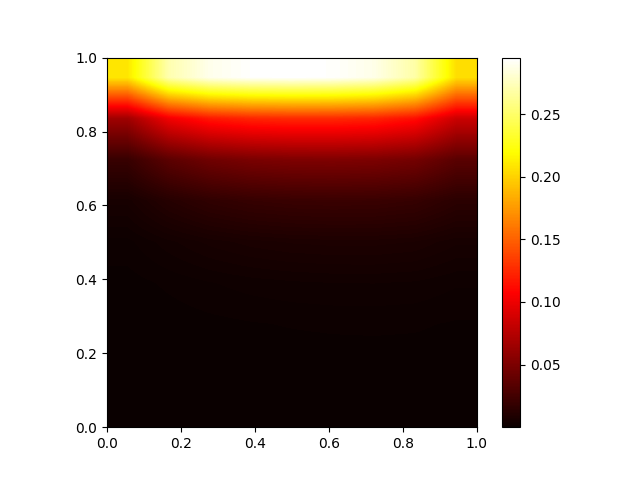
\includegraphics[width=0.5\textwidth]{images/mur_chaud.png}
  \caption{Résultat de la diffusion de température pour un mur chaud de température initiale 50°C placé au nord d'un plan non chauffé (avec une interpolation bilinéaire)}
  \label{fig:mur_chaud}
\end{figure}%

Nous pouvons constater que la température est de plus en plus proche de 0°C plus on s'éloigne du mur. De plus la température globale du mur a diminué. Donc la tendance générale des résultats obtenus est en adéquation avec le phénomène physique simulé.

\subsection{Résolution du système dans le cas d'un radiateur placé au centre}

Dans ce deuxième problème de la diffusion nous nous sommes intéressés à la diffusion de chaleur depuis un radiateur placé au centre d'un espace non chauffé. Ainsi notre vecteur de conditions initiales \texttt{b}  devient :
\begin{equation}\displaystyle{
  b=\begin{pmatrix} b_{1} = 0 \\ \vdots \\ b_{\dfrac{N^{2}+N}{2}-1} = 0 \\ b_{\dfrac{N^{2}+N}{2}} = -h^{2}T_{radiateur} \\
  b_{\dfrac{N^{2}+N}{2}+1} == 0 \\ \vdots \\ b_{N^{2}} = 0 \end{pmatrix}}
\end{equation}

En résolvant notre système avec la fonction \texttt{probleme\_radiateur\_centre} sur un plan de taille \texttt{N=9} et une température \texttt{$T_{radiateur}=50$} nous obtenons la figure ~\ref{fig:radiateur_centre} qui rend compte de la distribution de chaleur sur les points de notre plan obtenue grâce au vecteur image $x$ solution de $Ax=b$.

\begin{figure}[htbp]
  \centering
  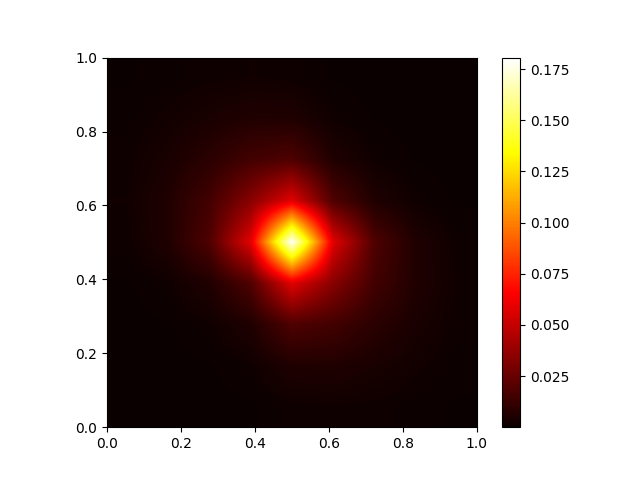
\includegraphics[width=0.5\textwidth]{images/radiateur_centre.png}
  \caption{Résultat de la diffusion de température pour un radiateur de température de départ à 50°C placé au centre du plan non chauffé (avec une interpolation bilinéaire)}
  \label{fig:radiateur_centre}
\end{figure}%

Nous pouvons observer que la température du radiateur a diminué et que la température baisse en fonction de la distance au radiateur. La figure ~\ref{fig:radiateur_centre} présente une bonne cohérence avec le phénomène physique simulé. Mais notre algorithme ne permet pas de rendre compte du phénomène de diffusion dans le cas où le radiateur marche en continu car dans ce cas précis sa température reste constante.







\section*{Conclusion}
Pour conclure, la méthode à utiliser pour la résolution d'un système linéaire en un temps raisonnable dépend grandement du contexte du problème. Dans notre cas nous avons constaté une différence non négligeable du temps de résolution d'un système linéaire selon son caractère plus ou moins creux et selon le nombre d'équations le constituant. De plus, nous avons remarqué que pour certains systèmes nous pouvons réduire leur temps de résolution avec un bon préconditionnement modulo une certaine marge d'erreur sur la solution finale. Pour finir l'application à la diffusion de chaleur en deux dimensions nous montre que de nombreux problèmes peuvent être approximés par un système d'équations linéaires dont la résolution peut donner des éléments de solutions ainsi qu'une tendance générale des résultats au problème donné.
\end{document}
